% Signal calculator notes: 2026-08-18. One canonical source for this exam.
% Current export: question 2(b), 68b-difference-equation.png.
% Original question: c2360b75-8986-11f0-817c-81fdb65741b1 - Omtentamen - Sundsvall.pdf,
% PDF page 2 (printed page 1), original-image crop (325,2180,2260,3230).
% Handwritten method: exaam/exaam/IMG_20261024_154103.jpg, dated 2026-08-18, 2B.
% Introductory support: IMG_20261024_154041.jpg and IMG_20261024_154120.jpg.
% Preserve the handwritten input-path -> feedback-path -> output-sum calculation.
% The brief system check follows the shared block-diagram family template.
\documentclass[10pt]{article}
\usepackage[T1]{fontenc}
\usepackage{lmodern}
\usepackage{amsmath}
\usepackage{graphicx}
\usepackage{microtype}
\usepackage[paperwidth=384bp,paperheight=1800bp,
  left=8bp,right=8bp,top=8bp,bottom=8bp]{geometry}
\pagestyle{empty}
\setlength{\parindent}{0pt}
\setlength{\parskip}{3pt}
\setlength{\abovedisplayskip}{4pt}
\setlength{\belowdisplayskip}{4pt}
\setlength{\abovedisplayshortskip}{3pt}
\setlength{\belowdisplayshortskip}{3pt}
\setlength{\jot}{3pt}
\raggedright
\newcommand{\noteheading}[1]{\par\vspace{6pt}\textbf{#1}\par}
\newcommand{\stepheading}[1]{\par\vspace{4pt}\textbf{#1}\par}

\begin{document}
{\fontsize{14}{17}\selectfont\textbf{Uppgift 2b}}\hfill
{\small 2026-08-18}\par
\textbf{Original question}\par
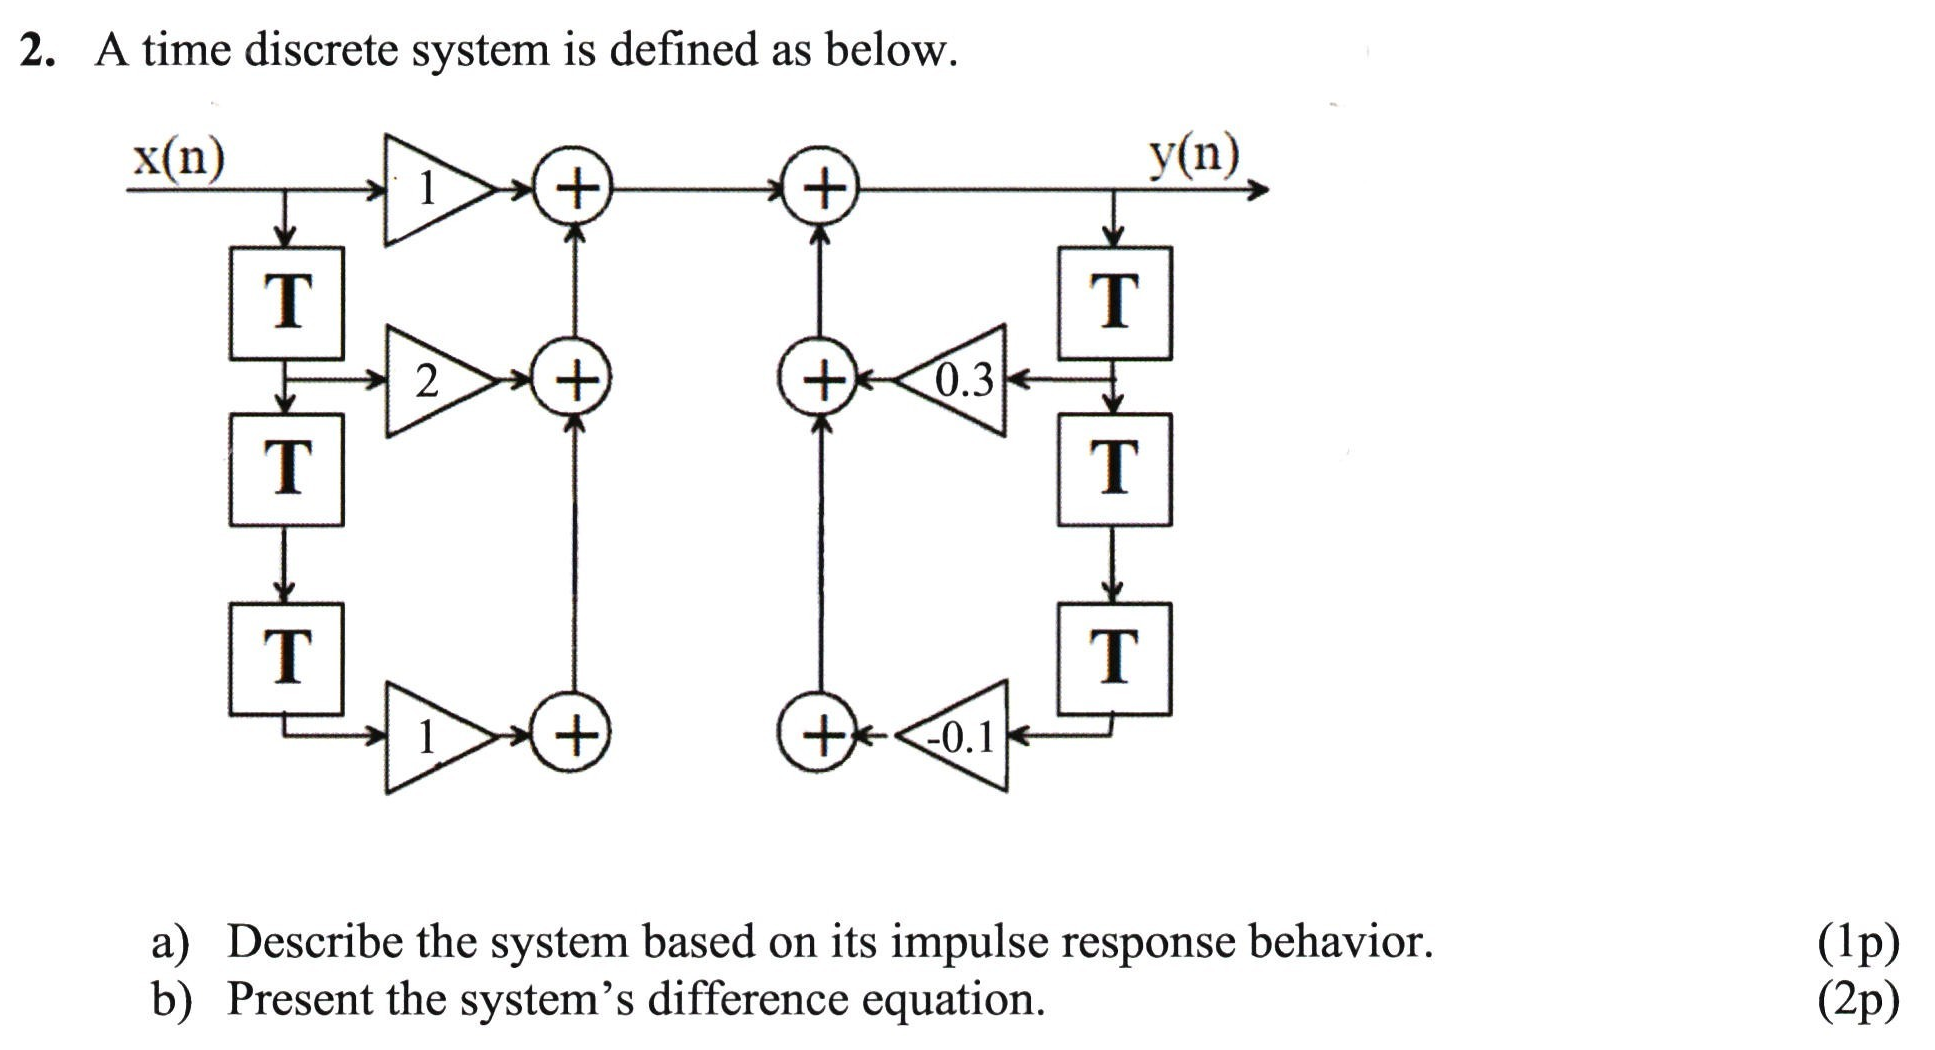
\includegraphics[width=\linewidth]{assets/68-q2-question.png}\par

\vspace{5pt}
{\fontsize{12}{15}\selectfont\textbf{Compiled notes}}\par

\noteheading{What we are doing}
We want the difference equation.
Read each path, then add the input and feedback terms.

\noteheading{Step-by-step solution}
\stepheading{1. Check delays and feedback}
Each $T$ delays the signal by one sample.\par
Previous outputs return to the sum, so there is feedback.
This feedback makes the system \textbf{IIR}.\par
Only present and past values are used, so it is \textbf{causal}.

\stepheading{2. Read the input paths}
Count the delays before each gain:
\[
\begin{aligned}
  0\text{ delays:}\quad &1\cdot x(n)=x(n)\\
  1\text{ delay:}\quad &2\cdot x(n-1)\\
  3\text{ delays:}\quad &1\cdot x(n-3)=x(n-3).
\end{aligned}
\]
There is no branch into the sum after the second $T$.
So there is no $x(n-2)$ term.\par
Add the three input terms:
\[
\begin{aligned}
\text{Input sum}
  &=x(n)+2x(n-1)\\
  &\quad+x(n-3).
\end{aligned}
\]

\stepheading{3. Read the feedback paths}
Now start from $y(n)$ and follow the return paths:
\[
\begin{aligned}
  1\text{ delay:}\quad &0.3y(n-1)\\
  3\text{ delays:}\quad &-0.1y(n-3).
\end{aligned}
\]
Again, there is no branch into the sum after the second $T$.
So there is no $y(n-2)$ term.\par
Keep the minus sign from the lower gain:
\[
\begin{aligned}
\text{Feedback sum}
  &=0.3y(n-1)\\
  &\quad-0.1y(n-3).
\end{aligned}
\]

\stepheading{4. Combine at the output}
The final $+$ adds the input sum and feedback sum.
So the output becomes:

\noteheading{Final answer for part b)}
\[
\boxed{\begin{aligned}
y(n)&=x(n)\\
    &\quad+2x(n-1)+x(n-3)\\
    &\quad+0.3y(n-1)\\
    &\quad-0.1y(n-3).
\end{aligned}}
\]

\noteheading{What to remember}
Count every $T$ before a branch enters a sum.
Keep the sign of each gain.
\end{document}
